\documentclass[t,svgnames]{beamer}
\usetheme[deutsch]{KIT}
\setbeamercovered{transparent}
\setbeamertemplate{navigation symbols}{}

\KITfoot{Worthwhile - Praxis der Softwareentwicklung WS 2011/2012}
\usepackage[utf8]{inputenc}
\usepackage{ngerman}
%\usepackage[svgnames]{xcolor}
\usepackage{listings}
\usenavigationsymbols

\lstdefinelanguage{worthwhile}
  {morekeywords={function,Boolean,Integer,_ensures,_return,return,_assert,_requires,_invariant,while,if},
   morekeywords={[2]true,false},
      sensitive=true,
  morecomment=[l]{//},
  morecomment=[s]{/*}{*/},
  morestring=[b]",
}


\lstset{
   basicstyle=\ttfamily,
   keywordstyle=\bfseries\ttfamily\color{KITgreen},
   keywordstyle={[2]\bfseries\ttfamily\color{KITblue}},
   stringstyle=\color{green}\ttfamily,
   commentstyle=\color{KITblack50}\ttfamily,
   emph={square}, 
   emphstyle=\color{blue}\texttt,
   emph={[2]root,base},
   emphstyle={[2]\color{yac}\texttt},
   showstringspaces=false,
   flexiblecolumns=false,
   tabsize=2,
   numbers=left,
   numberstyle=\scriptsize,
   numberblanklines=true,
   stepnumber=1,
   numbersep=10pt,
   xleftmargin=15pt,
   language=worthwhile
 }

\title{Worthwhile}
\subtitle{Abschlusspräsentation}
\author{Leon Handreke $\cdot$ Chris Hiatt $\cdot$ Stefan Orf $\cdot$ Joachim Priesner $\cdot$ Fabian Ruch $\cdot$ Matthias Wagner}

\institute[ITI]{Institut für Theoretische Informatik}

\TitleImage[trim=-24mm -35mm 0 0,width=0.9\titleimagewd]{logo.pdf}

\begin{document}

\begin{frame}
\maketitle
\end{frame}

\begin{frame}[fragile]
	\frametitle{Was machen wir?}
	
	\begin{itemize}
		\item \textbf{Programmverifikation:} Formaler Beweis, dass ein Programm seine Spezifikation erfüllt.
		\item Wichtig z.~B. für sicherheitskritische Systeme
		\item Unterstützt durch Software (Formel-Generierung, Beweistools)
	\end{itemize}
	
		
%	\begin{lstlisting}[frame=lines,mathescape=true]
%		function Boolean isEven(Integer i)
%		    _ensures _return = true $\Leftrightarrow $ i % 2 = 0
%		{
%		    if (i / 2) $ \cdot $ 2 = i {
%		        return true
%		    } else {
%		        return false
%		    }
%		}
%	\end{lstlisting}
	
	% \begin{center}$\Rightarrow$ $$\mathtt{\forall i \in \mathbb{N} : (i / 2 \cdot 2 = i \Rightarrow i \% 2 = 0) \wedge (\neg(i / 2 \cdot 2 = i) \Rightarrow \neg(i \% 2 = 0))}$$\end{center}
	
\end{frame}

\begin{frame}[fragile]
	\frametitle{Beispiel}
	
	\begin{onlyenv}<1>
	\begin{lstlisting}[frame=lines,mathescape=true]
		function Boolean isEven(Integer i)
		    _ensures _return = true $\Leftrightarrow $ i % 2 = 0
		{
		    if (i / 2) $ \cdot $ 2 = i {
		        return true
		        
		    } else {
		        return false
		        
		    }
		}
	\end{lstlisting}
	\end{onlyenv}
	
	\begin{onlyenv}<2>
	\begin{lstlisting}[frame=lines,mathescape=true]
		function Boolean isEven(Integer i)
		
		{
		    if (i / 2) $ \cdot $ 2 = i {
		        return true
		        _assert _return = true $\Leftrightarrow $ i % 2 = 0
		    } else {
		        return false
		        _assert _return = true $\Leftrightarrow $ i % 2 = 0
		    }
		}
	\end{lstlisting}
	\end{onlyenv}
	
	\begin{onlyenv}<3>
	\begin{lstlisting}[frame=lines,mathescape=true]
		function Boolean isEven(Integer i)
		
		{
		    if (i / 2) $ \cdot $ 2 = i {
		    
		        _assert    true = true $\Leftrightarrow $ i % 2 = 0
		    } else {
		    
		        _assert   false = true $\Leftrightarrow $ i % 2 = 0
		    }
		}
	\end{lstlisting}
	\end{onlyenv}
	
		\begin{onlyenv}<4>
	\begin{lstlisting}[frame=lines,mathescape=true]
		function Boolean isEven(Integer i)
		
		{
		    if (i / 2) $ \cdot $ 2 = i {
		        // hier gilt (i / 2) $ \cdot $ 2 = i
		        _assert    true = true $\Leftrightarrow $ i % 2 = 0
		    } else {
		        // hier gilt $\neg$((i / 2) $ \cdot $ 2 = i)
		        _assert   false = true $\Leftrightarrow $ i % 2 = 0
		    }
		}
	\end{lstlisting}
	\end{onlyenv}
	
		\begin{onlyenv}<5>
	\begin{lstlisting}[frame=lines,mathescape=true]
		function Boolean isEven(Integer i)
		
		{
		    _assert
		        (i / 2) $ \cdot $ 2 = i $\Rightarrow$
		                  (true = true $\Leftrightarrow $ i % 2 = 0)
		    $\wedge$    	
		        $\neg$((i / 2) $ \cdot $ 2 = i) $\Rightarrow$
		                 (false = true $\Leftrightarrow $ i % 2 = 0)
		        	
		}
	\end{lstlisting}
	\end{onlyenv}
	
	
		\begin{onlyenv}<6-7>
	\begin{lstlisting}[frame=lines,mathescape=true]
	
		        
		_assert $\forall$ i $\in \mathbb{Z} :$	  
		    
		        (i / 2) $ \cdot $ 2 = i $\Rightarrow$
		                  (true = true $\Leftrightarrow $ i % 2 = 0)
		    $\wedge$    	
		        $\neg$((i / 2) $ \cdot $ 2 = i) $\Rightarrow$
		                 (false = true $\Leftrightarrow $ i % 2 = 0)
		        	
		$~$
	\end{lstlisting}
	\end{onlyenv}
	
	\vspace{1cm}
	
	\only<7> {
		$\Rightarrow$ Diese Formel ist beweis- oder widerlegbar!
	}
\end{frame}

\begin{frame}
	\frametitle{Was ist Worthwhile?}

	\begin{columns}[c]
		\column{0.5 \textwidth}
			\begin{itemize}
			\item Eine WHILE-Sprache
			\end{itemize}
		\column{0.45 \textwidth}
	\end{columns}
\end{frame}

\lstset{
   basicstyle=\scriptsize\ttfamily
}

\begin{frame}[fragile]
	\frametitle{Was ist Worthwhile?}
	
	\begin{lstlisting}[frame=lines,mathescape=true]
/* Checks that the given array fulfils the heap condition. */
function Boolean heapCondition(Integer[] heap)
    _requires heapsize(heap) $\geq$ 0
    _ensures _return = $\forall$ Integer i1, 2 $\leq$ i1 $\wedge$ i1 $\leq$ heapsize(heap) : heap[parent(i1)] $\leq$ heap[i1]
{
    Boolean result := true
    
    if (heapsize(heap) $\geq$ 2) {
        Integer i3 := 2
        
        while i3 $\leq$ heapsize(heap)
            _invariant 2 $\geq$ i3 $\wedge$ i3 $\leq$ heapsize(heap) + 1
            
            // The invariant is that the contents of "result" indicate whether the
            // sub-array [1..i3-1] of the input fulfils the heap condition.
            _invariant result = $\forall$ Integer i4, 2 $\leq$ i4 $\wedge$ i4 $<$ i3 : heap[parent(i4)] $\leq$ heap[i4]
        {
            if result = true {
                if heap[parent(i3)] $>$ heap[i3] {
                    result := false
                }
            }
    \end{lstlisting}
\end{frame}

\begin{frame}
	\frametitle{Was ist Worthwhile?}

	\setbeamercovered{invisible}
	\begin{columns}[c]
		\column{0.5 \textwidth}
		\begin{itemize}
			\item Eine WHILE-Sprache
			\uncover<2->{\item Eine Entwicklungsumgebung
					\begin{itemize}
						\item Editor
						\item Interpreter
						\item Debugger
					\end{itemize}
				}
			\uncover<3->{\item Ein Formelgenerator}
		\end{itemize}

		\column{0.45 \textwidth}

		\begin{figure}
			\uncover<2->{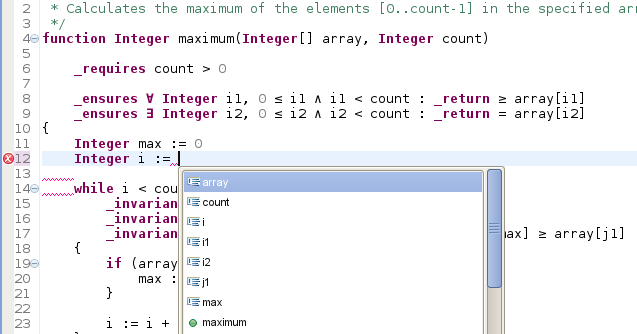
\includegraphics[width=\textwidth]{screenshot1.png}}
		\end{figure}

	\end{columns}

	\begin{columns}[c]
		\column{0.5 \textwidth}
		\begin{itemize}
			\uncover<4->{\item Beweiserschnittstelle
				\begin{itemize}
				\item Aufruf des Beweisers  \\ {\scriptsize \vspace{-0.08cm} (Beweiser ist \textbf{externes} Tool)} \vspace{0.02cm}}
						\uncover<5->{
						\item Rückmeldung für Benutzer  \\ {\scriptsize \vspace{-0.08cm} Wo schlägt der Beweis fehl? \vspace{0.02cm}
						}}
				\end{itemize}
		\end{itemize}

		
		
		\column{0.45 \textwidth}

\begin{onlyenv}<4>
		\begin{figure}
			
\includegraphics[width=\textwidth]{z3.png}
		\end{figure}
		
	\end{onlyenv}
	
			\begin{onlyenv}<5>

		\begin{figure}
			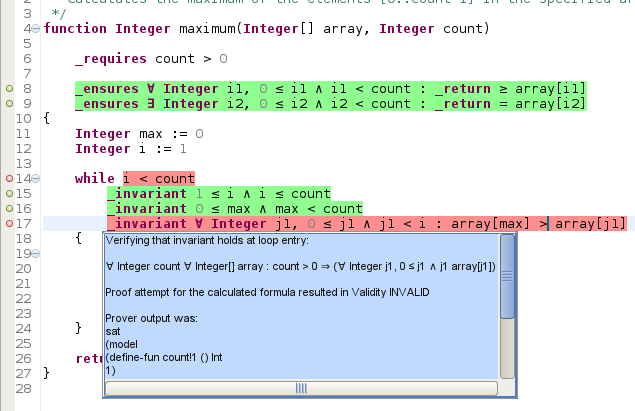
\includegraphics[width=\textwidth]{screenshot2.png}
		\end{figure}
	\end{onlyenv}
	
		\end{columns}

	\setbeamercovered{transparent}

\end{frame}


\begin{frame}
	\begin{center}
		\vfill
		\Huge{DEMO}
		\vfill		
	\end{center}
\end{frame}

\begin{frame}
    \frametitle{Erfahrungen}
    \begin{itemize}
        \item Es gibt sehr gut anwendbare Frameworks: Eclipse/Xtext
        \item Unterstützung durch/Erfahrung mit Tools (Git, Mailingliste, Wiki, IDE)
        \item Empirischer Beweis des Sinns von Softwaretechnik
    \end{itemize}
    \begin{itemize}
        \item Nur wenig geeignete UML-Modellierungstools: fehlende Versionierung
        \item Einschränkungen von Java (z.\,B.\ Visitor-Implementierung)
        \item Wasserfallmodell ungeeignet
        \begin{itemize}
            \item Prototypentwicklung nicht vorgesehen
            \item Dokumente am Ende jeder Phase wenig nutzvoll
            \item Rückkopplung nicht vorgesehen
        \end{itemize}
    \end{itemize}
\end{frame}

\begin{frame}
    \frametitle{Zukunft des Projekts}
    \begin{itemize}
        \item Öffentliches Repository auf Github mit Bugtracker
        \item 3-Clause-BSD-Lizenz
    \end{itemize}
\end{frame}

\end{document}
